% !TEX program = xelatex
\documentclass[UTF8,a4paper,12pt]{ctexart}

% 基本版式(单栏)
\usepackage[margin=2.2cm]{geometry}
\usepackage{setspace}
\onehalfspacing

% 断行与微排版
\usepackage{ragged2e}
\usepackage[protrusion=true,expansion=false]{microtype}
\microtypecontext{spacing=nonfrench}
\setlength{\emergencystretch}{3em}
\sloppy

% 数学宏包
\usepackage{amsmath, amssymb, amsfonts, mathtools}
\allowdisplaybreaks[2]
\numberwithin{equation}{section}

% 表格与布局
\usepackage{tabularx, booktabs, array}
\newcolumntype{Y}{>{\RaggedRight\arraybackslash}X}
\newcolumntype{C}{>{\centering\arraybackslash}X}

% 字体(ctex 已处理中文;英文字体可按需微调)
\usepackage{fontspec}
\setmainfont{Times New Roman}
\setsansfont{Arial}
\setmonofont{Consolas}

% 颜色与盒子
\usepackage[dvipsnames]{xcolor}
\usepackage[most]{tcolorbox}
\tcbset{colback=white,colframe=MidnightBlue!60!black,boxrule=0.6pt,arc=2pt}

% 图形绘制(TikZ / PGFPlots)
\usepackage{tikz}
\usetikzlibrary{arrows.meta,calc,positioning}
\usepackage{pgfplots}
\pgfplotsset{compat=1.18}

% 超链接
\usepackage[colorlinks=true,linkcolor=blue,citecolor=blue,urlcolor=blue]{hyperref}

% 标题信息
\title{伽马函数(Gamma Function)速记与例题(单栏速查版)}
\author{\small 摘要整理}
\date{\small \today}

\begin{document}
\maketitle

\section{定义与基本性质}
伽马函数将阶乘从正整数延拓至非整数乃至复数域,经典定义(欧拉第二类积分)为
\begin{equation}
\Gamma(x) = \int_0^{\infty} t^{x-1} e^{-t} \, dt,\quad \Re(x)>0.
\end{equation}
与阶乘、常用性质:
\begin{itemize}
  \item 递推:\(\Gamma(x+1) = x\,\Gamma(x)\)
  \item 正整数:\(\Gamma(n+1) = n!\)(如 \(\Gamma(4)=3!=6\))
  \item 关键特值:\(\Gamma(\tfrac{1}{2}) = \sqrt{\pi}\)
  \item 与 Beta 函数:
  \begin{equation}
    B(x,y) = \int_0^1 t^{x-1} (1-t)^{y-1} \, dt
    = \frac{\Gamma(x)\,\Gamma(y)}{\Gamma(x+y)}.
  \end{equation}
  \item 指数积分模板:
  \begin{equation}
    \int_0^{\infty} x^{p-1} e^{-a x} \, dx = \frac{\Gamma(p)}{a^p},\qquad a>0,\ \Re(p)>0.
  \end{equation}
  \item 反射公式(了解):
  \begin{equation}
    \Gamma(x)\,\Gamma(1-x) = \frac{\pi}{\sin(\pi x)}.
  \end{equation}
\end{itemize}

\section{历史小结}
从“如何把阶乘扩展到非整数”的问题出发,伽马函数在 18–19 世纪逐步定型:
\begin{itemize}
  \item 1720s:伯努利与哥德巴赫讨论“延拓阶乘”的问题。
  \item 1729–1730:欧拉给出无穷乘积与积分形式解法,称为“第二类欧拉积分”。
  \item 1808 前后:勒让德引入记号 \(\Gamma(x)\) 并命名为“伽马函数”。
  \item 19 世纪:高斯、魏尔斯特拉斯等拓展其在复分析与数论中的性质与应用。
\end{itemize}

\section{常见记忆要点}
\begin{itemize}
  \item 看到 \(\int_0^{\infty} x^m e^{-a x^k} dx\) 型,常以代换“凑”成 \(\Gamma\) 形式。
  \item \(\Gamma(\tfrac{1}{2}) = \sqrt{\pi}\) 与递推 \(\Gamma(z+1) = z\,\Gamma(z)\) 常联用。
  \item 与 Beta 函数互化:区间 \([0,1]\) 的幂函数积分 \(\leftrightarrow\) \(\Gamma\) 比例。
\end{itemize}

\section{例题:用伽马函数求积分(详细步骤)}
设 \(f(x) = \dfrac{4x^2}{a^3\sqrt{\pi}} e^{-x^2/a^2}\) 当 \(x>0\),且 \(f(x)=0\) 当 \(x\le 0\)。求 \(I = \int_{-\infty}^{+\infty} x^2 f(x)\,dx\)。
\subsection*{步骤1:改写积分}
因 \(f(x)=0\)(\(x\le 0\)),故
\begin{align}
I &= \int_0^{+\infty} x^2\Big(\frac{4x^2}{a^3\sqrt{\pi}} e^{-x^2/a^2}\Big) dx\\
  &= \frac{4}{a^3\sqrt{\pi}} \int_0^{+\infty} x^4 e^{-x^2/a^2} dx.
\end{align}
\subsection*{步骤2:关键代换以“凑”标准型}
令 \(t = x^2/a^2\)(\(x = a\sqrt{t}\)),则 \(dx = \dfrac{a}{2\sqrt{t}} dt\),且 \(x^4 = a^4 t^2\)。代回得
\begin{align}
\int_0^{+\infty} x^4 e^{-x^2/a^2} dx
&= \int_0^{+\infty} a^4 t^2 e^{-t} \cdot \frac{a}{2\sqrt{t}} dt\\
&= \frac{a^5}{2} \int_0^{+\infty} t^{3/2} e^{-t} dt.
\end{align}
\subsection*{步骤3:识别伽马函数}
与定义 \(\Gamma(z) = \int_0^{\infty} t^{z-1} e^{-t} dt\) 对比,取 \(z-1=\tfrac{3}{2}\Rightarrow z=\tfrac{5}{2}\),故
\(\int_0^{+\infty} t^{3/2} e^{-t} dt = \Gamma(\tfrac{5}{2})\)。
\subsection*{步骤4:合并并计算数值}
\begin{align}
I &= \frac{4}{a^3\sqrt{\pi}} \cdot \frac{a^5}{2} \cdot \Gamma\!\Big(\tfrac{5}{2}\Big)
= \frac{2a^2}{\sqrt{\pi}}\,\Gamma\!\Big(\tfrac{5}{2}\Big).
\end{align}
又由 \(\Gamma(\tfrac{5}{2}) = \tfrac{3}{2}\,\Gamma(\tfrac{3}{2}) = \tfrac{3}{2}\cdot\tfrac{1}{2}\,\Gamma(\tfrac{1}{2}) = \tfrac{3}{4}\sqrt{\pi}\),得
\(I = \dfrac{2a^2}{\sqrt{\pi}}\cdot \dfrac{3}{4}\sqrt{\pi} = \dfrac{3}{2}a^2\)。

\section{图表与示意}
\subsection*{作用速览(应用领域 × 典型形式)}
\begin{tcolorbox}
\small
\setlength{\tabcolsep}{4pt}
\begin{tabularx}{\linewidth}{@{}Y Y@{}}
\toprule
\textbf{领域} & \textbf{典型形式 / 用途} \\
\midrule
概率统计 & $\Gamma(\tfrac{1}{2})=\sqrt{\pi}$;正态积分;伽马/卡方分布密度与矩 \\
积分计算 & $\int_0^{\infty} x^{p-1} e^{-a x} dx = \Gamma(p)/a^p$;换元“凑”$\Gamma$ \\
级数与乘积 & 魏尔斯特拉斯乘积、反射公式;黎曼$\zeta$与$\Gamma$联系(了解) \\
组合延拓 & $n!\to\Gamma(n+1)$ 将阶乘推广至非整数 \\
微分方程 & 通过$\Gamma$与$B$函数求常见积分特解 \\
机器学习 & 共轭先验:Gamma/Dirichlet \\
\bottomrule
\end{tabularx}
\end{tcolorbox}

\subsection*{数值表与形状印象($x>0$)}
\begin{tcolorbox}
\small
\setlength{\tabcolsep}{6pt}
\begin{tabularx}{\linewidth}{@{}C C C C C C C@{}}
\toprule
$x$ & $0.5$ & $1$ & $1.5$ & $2$ & $3$ & $4$ \\
\midrule
$\Gamma(x)$ & $1.772$ & $1$ & $0.886$ & $1$ & $2$ & $6$ \\
\bottomrule
\end{tabularx}
\end{tcolorbox}

在区间 $((0, +\infty))$ 上,$\Gamma(x)$ 在 $x\approx 1.4616$ 附近有极小值(约 $0.8856$),随后随 $x$ 增大迅速增长;并在 $x=1,2,3,4,\ldots$ 取到 $1!,2!,3!,4!$。

\subsection*{曲线示意(TikZ/PGFPlots)}
\begin{tcolorbox}
\centering
\begin{tikzpicture}
  \begin{axis}[
    width=0.9\linewidth,
    height=6cm,
    xmin=0,xmax=5,
    ymin=0,ymax=6.5,
    grid=both,
    grid style={gray!20},
    axis lines=left,
    xlabel={$x$},ylabel={$\Gamma(x)$},
    tick align=outside,
    legend style={draw=none,at={(0.02,0.98)},anchor=north west,font=\scriptsize}
  ]
    \addplot[smooth,thick,MidnightBlue] coordinates {
      (0.20,4.5908)
      (0.30,3.5720)
      (0.40,2.9550)
      (0.50,1.7725)
      (0.60,1.4892)
      (0.80,1.1642)
      (1.00,1.0000)
      (1.20,0.9182)
      (1.40,0.8873)
      (1.46,0.8856)
      (1.60,0.8935)
      (1.80,0.9314)
      (2.00,1.0000)
      (2.50,1.3293)
      (3.00,2.0000)
      (3.50,3.3234)
      (4.00,6.0000)
      (4.50,11.6317)
      (5.00,24.0000)
    };
    \addlegendentry{$\Gamma(x)$}
    \addplot[only marks,mark=*,mark size=1.6pt,red] coordinates {(1.4616,0.8856)};
    \node[anchor=south west,red] at (axis cs:1.5,0.95) {\scriptsize 极小值};
  \end{axis}
\end{tikzpicture}
\end{tcolorbox}

\subsection*{收敛域示意}
\begin{tcolorbox}
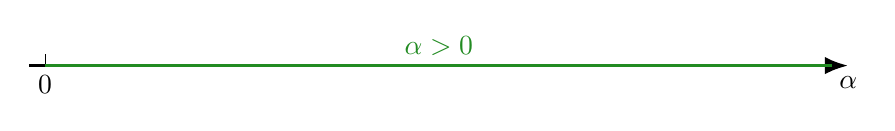
\begin{tikzpicture}
  \draw[very thick,-{Latex}] (-0.2,0) -- (10.2,0) node[below]{$\alpha$};
  \draw (0,0) node[below]{0} -- (0,0.15);
  \draw[very thick,ForestGreen] (0,0) -- (10,0);
  \node[above,ForestGreen] at (5,0) {$\alpha>0$};
\end{tikzpicture}
\end{tcolorbox}

\section{核心问题:$\Gamma(\alpha)$ 的敛散性}
我们要判断积分 \(\Gamma(\alpha) = \int_0^{+\infty} x^{\alpha-1} e^{-x} dx\) 在 \(\alpha\) 取何值时收敛。考虑两个可能的瑕点:$x\to 0^+$ 与 $x\to +\infty$。在 $x=1$ 处分割:
\begin{equation}
\Gamma(\alpha) = \underbrace{\int_0^1 x^{\alpha-1} e^{-x} dx}_{I_1} + \underbrace{\int_1^{+\infty} x^{\alpha-1} e^{-x} dx}_{I_2}.
\end{equation}

\subsection*{1. $I_2 = \int_1^{+\infty} x^{\alpha-1} e^{-x} dx$($x\to+\infty$ 处)}
用极限比较审敛法,与 \(g(x)=1/x^2\) 比较(其在 $[1,\infty)$ 上可积)。
\begin{equation}
\lim_{x\to+\infty} \frac{x^{\alpha-1} e^{-x}}{1/x^2} = \lim_{x\to+\infty} \frac{x^{\alpha+1}}{e^x} = 0,
\end{equation}
由多次洛必达法则可证。故 $I_2$ 对任意实数 $\alpha$ 均收敛。

\subsection*{2. $I_1 = \int_0^1 x^{\alpha-1} e^{-x} dx$($x\to 0^+$ 处)}
当 $x\to 0^+$,$e^{-x}\to 1$,决定敛散性的主要是 $x^{\alpha-1}$。比较 \(f(x)=x^{\alpha-1} e^{-x}\) 与 \(g(x)=x^{\alpha-1}\):
\begin{equation}
\lim_{x\to 0^+} \frac{x^{\alpha-1} e^{-x}}{x^{\alpha-1}} = \lim_{x\to 0^+} e^{-x} = 1.
\end{equation}
因此 $I_1$ 的敛散性与 $\int_0^1 x^{\alpha-1} dx$ 相同,而 \(\int_0^1 x^{\alpha-1} dx\) 收敛当且仅当 $\alpha>0$。

\subsection*{最终结论}
要使 $\Gamma(\alpha)$ 收敛,需 $I_1$ 与 $I_2$ 同时收敛:$I_2$ 对任意 $\alpha$ 收敛;$I_1$ 当且仅当 $\alpha>0$ 收敛。故
\begin{equation}
\boxed{\text{$\Gamma(\alpha)$ 的收敛域为 }\ \alpha>0.}
\end{equation}

\end{document}

